\documentclass[margin,line]{res}
\usepackage[utf8]{inputenc}
\usepackage{multirow}
\usepackage{graphicx}

\oddsidemargin -.5in
\evensidemargin -.5in
\textwidth=6.0in
\itemsep=0in
\parsep=0in

\newenvironment{list1}{
  \begin{list}{\ding{113}}{%
      \setlength{\itemsep}{0in}
      \setlength{\parsep}{0in} \setlength{\parskip}{0in}
      \setlength{\topsep}{0in} \setlength{\partopsep}{0in} 
      \setlength{\leftmargin}{0.17in}}}{\end{list}}
\newenvironment{list2}{
  \begin{list}{$\bullet$}{%
      \setlength{\itemsep}{0in}
      \setlength{\parsep}{0in} \setlength{\parskip}{0in}
      \setlength{\topsep}{0in} \setlength{\partopsep}{0in} 
      \setlength{\leftmargin}{0.2in}}}{\end{list}}


\begin{document}

\name{Óscar Andrés Nájera Ocampo}

\begin{resume}

\section{\sc Contact Information}
  \begin{tabular}{@{}p{2in}p{2.5in}p{3cm} }
    {\it Home Address:}    &  &
      \multirow{4}{*}{ 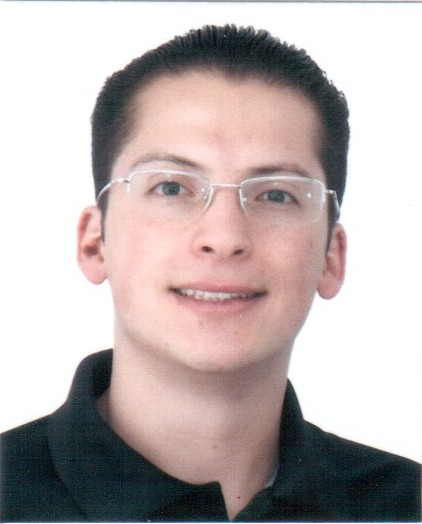
\includegraphics[width=3cm,bb=0 0 101 126]{./foto2012.jpg}}\\

    62, Rue Camille Desmoulins & {\it mobile:} (+33) 0750908406 \\
    CH 248 Bât G      & {\it e-mail:}  najera.oscar@gmail.com\\
    94234 Cachan Cedex, France    & {\it www:} http://titan-c.github.com
  \end{tabular}\vspace{0.4cm}

\section{\sc Personal Information}
 \begin{tabular}{ll}
  {\it Family Name:} Nájera Ocampo & {\it Date of Birth:} 13 April 1988\\
  {\it Given Name:} Óscar Andrés   & {\it Gender:} Male\\
  {\it Nationality:} Ecuadorian    & %{\it Marital status:} Single
 \end{tabular}

\section{\sc Research Interests}
  Condensed Matter, Solid State Physics, Statistical Mechanics, Mathematical \& Theoretical Physics, Scientific Programming \& computational systems analysis

\section{\sc Education}
  {\bf École Normale Supérieure de Cachan}, Cachan, France\\
  \vspace{-.1in}
  \begin{list1}
    \item[] M2 Master in Molecular Nano- bio-photonics (MONABIPHOT) \hfill 
{\bf Sept. 2013 - Present}
  \end{list1}

  {\bf Escuela Politécnica Nacional}, Quito, Ecuador\\
  \vspace{-.1in}
  \begin{list1}
    \item[] Physics Diploma \hfill {\bf Oct. 2006 - Sept. 2012}\\
    \begin{list2}
    \vspace{-.1in}
      \item[] {\bf $4^{th}$ best graduate among all 148 graduates on
      commencement day}
      \item Thesis Topic:  ``Estimation, by computer simulation, of the exchange
	energy dispersion between polar nano-regions in $Pb_xBi_4Ti_{3+x}O_{12+3x}; x=\{2,3\}$
	relaxor ferroelectrics''
%       \item Advisor: Dr. Luis Lascano
%       \item Written in: Spanish
%       \item Coursework grades: 8.2/10 | Written thesis: 9.8/10 | Oral 
% examination: 10/10
    \end{list2}
  \end{list1}

  {\bf German School}, Quito, Ecuador\\
  \vspace{-.1in}
  \begin{list1}
    \item[] German Abitur \hfill {\bf May 2006}
    \item[] Ecuadorian High School Diploma \hfill {\bf June 2005}
  \end{list1}

\section{\sc Honors and Awards}
  Paris-Saclay Master Scholarship, Campus Paris-Saclay, France \hfill {\bf
2013}\\
  Danced for Ecuador in WDSF World DanceSport Championship Standard, Australia \hfill {\bf 2012}\\
  Physics Olympiad $1^{st}$ place, Escuela Politécnica Nacional, Ecuador \hfill {\bf 2010}\\
  Bronze Medal for Academic performance, German School Quito, Ecuador \hfill {\bf 2005}\\
  PAD Preisträger, Kultusminister Konferenz, Germany \hfill {\bf 2003}

\section{\sc Academic Experience}
  {\bf Université Paris Sud}, Orsay, France
  \begin{list1}
    \item[] {\em M2 Internship at Laboratoire de Physique des Solides} 
\hfill {\bf Feb. 17 2014 - Present, 2014}\\
Study of spin-orbit effects in the Mott-Hubbard metal-insulator transition
  \end{list1}
  
  {\bf Swiss Federal Institute of Technology(ETH)}, Zurich, Switzerland
  \begin{list1}
    \item[] {\em Visitor at Institute for Building Materials (IfB)} \hfill {\bf 
Apr. 5 - May 15, 2013}\\
    Training in Lattice Boltzmann Methods for fluid dynamics
  \end{list1}

  {\bf International Center for Theoretical Physics}, Trieste, Italy
  \begin{list1}
    \item[] {\em Teaching Assistant} \hfill {\bf Mar. 10 - 21, 2014} \\
    ``Workshop on Advanced Techniques for Scientific Programming and 
Management of Open Source Software packages'' SMR 2574
    \item[] {\em Invited Student} \hfill {\bf Mar. 11 - 22, 2013} \\
    ``Workshop on Computer Programming and Advanced Tools for Scientific
    Research Work'' SMR 2503
    \item[] {\em Invited Student} \hfill {\bf Feb. 20 - Mar. 2, 2012} \\
    ``Advanced School on Scientific Software Development'' SMR 2330
  \end{list1}

  {\bf Universidad Central del Ecuador}, Quito, Ecuador
  \begin{list1}
    \item[] {\em Trainee in the Molecular Symmetries and Quantum Chemistry Group} \hfill {\bf Oct. 2012 - Mar. 2013}
  \end{list1}

  {\bf Escuela Politécnica Nacional}, Quito, Ecuador
  \begin{list1}
%    \item[] {\em Student} \hfill {\bf Oct. 2006 - Sept. 2012}\\
%     Includes research and coursework\\
   \item[] {\em Laboratory and teacher's Assistant} \hfill {\bf Aug. 2011 - June 2012}\\
    Responsible of Experimental Physics laboratory in subjects
    like Newtonian Mechanics, Electromagnetism and Optics.
    Shared responsibility for lectures, homework assignments and grades in this subjects.\\
   \item[] {\em Teacher's Assistant} \hfill {\bf Sept. 2010 - Feb. 2011}\\
    Support students in single- \& multi-variable Calculus, and Real Analysis through
    exercise sessions and solutions of exams.
  \end{list1}

\section{\sc Conference Presentations}
  {\bf O. Nájera}, L. Lascano: ``Estimation of the exchange interaction dispersion between polar
  nano-regions in relaxors P2BIT \& P3BIT'', {\bf In:} XVI ELAVIO, {\em Latin American School in Operations Research}, Bento Gonçalves - RS - Brazil Feb. 2012.

\section{\sc Posters}
  {\bf O. Nájera}, L. Lascano: ``Estimation of the exchange interaction dispersion between PNR in
  relaxor ferroelectrics'',  Awarded poster {\bf In:} NanoAndes, Quito-Ecuador Nov. 2012

\section{\sc Other Publications}
  {\bf O. Nájera}: ``Estimation, by computer simulation, of the exchange energy dispersion between
  polar nano-regions in $Pb_xBi_4Ti_{3+x}O_{12+3x}; x=\{2,3\}$ relaxor ferroelectrics'', Diploma
  Thesis(Spanish). {\em Department of Physics - Escuela Politécnica Nacional}, Sept. 2012.

\section{\sc Computer Skills}
  \begin{list2}
    \item Programming Languages:  C/C++, Python, Bash, Php, Matlab/Octave
    \item Libraries \& packages: GSL, SciPy, NumPy
    \item Content-description languages: \LaTeX, HTML, CSS
    \item Operating Systems:  Linux(Gentoo \& Arch \& Ubuntu)
    \item Graphic design: Gimp, Inkscape, Blender
  \end{list2}

\section{\sc Languages}
  \begin{list2}
    \item English: Fluent
    \item German: Fluent
    \item Spanish: Native
    \item French: Intermediate
  \end{list2}
  
\section{\sc Personal Referees}
 \begin{list1}
  \item[] Dr. Luis Lascano
  \begin{list2}
   \item {\it e-mail:} luis.lascano@epn.edu.ec
   \item {\it Institution:} Escuela Politécnica Nacional
   \item Thesis supervisor \& Solid State Physics teacher EPN
  \end{list2}
 \end{list1}
%  
%  \begin{list1}
%   \item[] Dr. Federico Trigo
%   \begin{list2}
%    \item {\it e-mail:} federico.trigo@parisdescartes.fr
%    \item {\it Institution:} Laboratoire de Physiologie Cérébrale - Université 
% Paris Descartes
%    \item Professor in ``From neurons to neural networks''
%   \end{list2}
%  \end{list1} 
 
 \begin{list1}
  \item[] Prof. Dr Joseph Zyss
  \begin{list2}
   \item {\it e-mail:} joseph.zyss@lpqm.ens-cachan.fr
   \item {\it Institution:}  École Normale Supérieure de Cachan
   \item Teacher in Light matter interations: lasers
  \end{list2}
 \end{list1}
 
%   \begin{list1}
%   \item[] Dr. Marco Bayas
%   \begin{list2}
%    \item {\it e-mail:} marco.bayas@epn.edu.ec
%    \item {\it Institution:} Escuela Politécnica Nacional
%    \item Biophysics \& Computational Physics teacher EPN
%   \end{list2}
%  \end{list1}
%  
%  \begin{list1}
%   \item[] Dr. Luis Miguel Torres
%   \begin{list2}
%    \item {\it e-mail:} luis.torres@epn.edu.ec
%    \item {\it Institution:} Escuela Politécnica Nacional
%    \item Linear and Integer Programming teacher | Vice-dean of the School of Sciences
%   \end{list2}
%  \end{list1}

%  \begin{list1}
%   \item[] Dr. Edy Ayala
%   \begin{list2}
%    \item {\it e-mail:} edy.ayala@epn.edu.ec
%    \item {\it Institution:} Escuela Politécnica Nacional
%    \item Modern Physics \& Nuclear Physics teacher | Head of the Physics
% Department EPN
%   \end{list2}
%  \end{list1}
 
%  \begin{list1}
%   \item[] Dr. Germán Rojas
%   \begin{list2}
%    \item {\it e-mail:} german.rojas@epn.edu.ec
%    \item {\it Institution:} Escuela Politécnica Nacional
%    \item Functional Analysis teacher
%   \end{list2}
%  \end{list1}

%  \begin{list1}
%   \item[] Dr. Leonardo Basile
%   \begin{list2}
%    \item {\it e-mail:} leonardo.basile@epn.edu.ec
%    \item {\it Institution:} Escuela Politécnica Nacional
%    \item Thesis examination committee \& teacher Statistical Physics
%   \end{list2}
%  \end{list1}


\section{\sc Outside Interests}
 \begin{list2}
  \item Ballroom Dancing
  \item Cycling
  \item Swimming
 \end{list2}

\end{resume}
\end{document}
